\begin{abstract}
Cell conditioning in arbitrary-scale super-resolution can improve average
quality while harming individual images or frequency bands. We connect
failure diagnosis to a controlled test of how feature corrections are
allocated. A frozen-cohort replication on 32 natural images, LTE and an
LTE-derived experimental variant (SC-INR), under two inherited training
seeds finds harm against zero and nonzero cell references. An exact
squared-error decomposition separates overshoot from wrong-direction
corrections, which positive output attenuation cannot turn beneficial.
On a fixed $\times4$ synthetic grid, we trace 16 SC wrong-direction cases.
Restoring scale weights from a paired input rescues only one.
In a separately frozen follow-up, replacing selective attenuation by
uniform feature attenuation at exactly the native total feature-step norm
restores positive middle-band gain in all 16 cases. This persists with
zero-cell decoder ReLU gates frozen. Across all 32 middle-frequency
conditions, the intervention makes every gain positive, including the
31 originally harmful cases. Yet it harms all 16 low-frequency controls
in centre-region RGB. These results locate a content-dependent allocation
failure in the specified model and probes, rather than establish a
universal repair rule. Full-image RGB improvement in the focal cases is
small: a median 0.40\% MSE reduction over native conditioning.
\end{abstract}
\begin{keywords}
Arbitrary-scale super-resolution, cell conditioning, feature allocation,
controlled failure diagnosis
\end{keywords}

\section{Introduction and Related Work}
\label{sec:intro}
Arbitrary-scale super-resolution (ASISR) predicts image values at continuous
coordinates. LIIF supplies target cell size to a local decoder
\cite{chen2021liif}; LTE introduces cell-dependent phase estimation
\cite{lee2022lte}. These inputs specify the requested scale but do not
guarantee that the resulting correction improves reconstruction.
We ask: \emph{can harmful cell corrections be explained only by their
magnitude or decoder gate changes, or does allocation across latent
features matter?} We first distinguish failure types, then intervene on
the feature allocation of a specified failure class.

Harmful cell effects are not new. LIIF varies cell at fixed queries;
IPE-LIIF integrates positional features and reports cases where adding
cell hurts \cite{liu2021ipe}. Thera supplies analytic Gaussian filtering
and discusses mismatch with bicubic training \cite{becker2025thera}.
Integrating latent features need not equal integrating a nonlinear
decoder's RGB output. We diagnose inherited checkpoints, rather than
benchmark performance against these methods.

Frequency-resolved analysis includes HyRA's linear and nonlinear responses
\cite{fsds2024}, texture error analysis \cite{magid2022texture}, sinusoidal
probes \cite{kawai2026frequency}, and Nyquist-normalised forecasting
\cite{wang2026scaleanchoring}. Phase beyond spectral magnitude is classical
\cite{oppenheim1981phase}. We claim neither these principles nor the
quadratic identity below as new. Unlike architecture/retraining benchmarks
\cite{nasir2026empirical}, we test fixed-parameter interventions.

Our contribution is a bounded empirical chain: paired natural-image
measurements establish failure types and their scale; controlled inputs
identify a repeatable wrong-direction class; and a native-norm-matched
feature intervention restores its gain even with decoder gates frozen.
A low-frequency counterexample shows that the same intervention cannot
universally replace selective conditioning.

\section{Models and Failure Diagnosis}
\label{sec:recovery}
\subsection{Fixed comparison and model lineage}
Changing cell while holding LR observation, query and HR target fixed is
a conditioning intervention, not a physical change of pixel footprint.
Native cell does not certify an exact pixel integral.
LTE and SC inherit an EDSR-baseline encoder, DIV2K training
\cite{agustsson2017div2k}, a 256-dimensional representation, three
256-unit ReLU hidden layers and 1000 epochs at $\times1$--$\times4$.
SC-INR is our earlier LTE-derived experimental variant, not an independent
model family or a new method proposed here. LTE conditions Fourier phase
on cell. SC predicts frequency $\omega_k$ and phase from image features,
then weights sine/cosine features by
\begin{equation}
 W_k(c_{\rm rel})=\operatorname{sinc}(\omega_{kx}c_{{\rm rel},x}/2)
                 \operatorname{sinc}(\omega_{ky}c_{{\rm rel},y}/2),
 \label{eq:sc}
\end{equation}
where $\operatorname{sinc}(v)=\sin(\pi v)/(\pi v)$ and
$c_{\rm rel}=c\,n_{\rm LR}$. Its 128 frequencies use signed $2.1\tanh$
parameterisation. Cell enters only through $W$ before the MLP, not the
feature-predicted phase. Frequency/phase parameterisations also differ
between LTE and SC, so cross-model quality cannot isolate sinc's effect.

A retrained no-cell ablation changes weights; our interventions do not.
The natural-image replication uses inherited seeds 1 and 2; controlled
probes use seed1. LTE snapshots omit the original extrapolation cell clamp.
Zero cell is outside training support. Nonzero references test whether
harm is confined to that contrast.

\subsection{Overshoot, direction and the object being changed}
For native prediction $F_c$, reference $F_r$, HR target $t$ and
$d=F_c-F_r$, set $a=\langle t-F_r,d\rangle$ and $b=\|d\|^2$.
Inner products are pixel/channel means, optionally after band projection.
\begin{equation}
 G(\lambda)=\operatorname{MSE}(F_r,t)-\operatorname{MSE}(F_r+\lambda d,t)
            =2\lambda a-\lambda^2b.
 \label{eq:gain}
\end{equation}
For harmful $G(1)<0$, $0<a<b/2$ is \emph{overshoot}: a smaller positive
correction can help. If $a<0$, the \emph{direction is wrong}: every
positive multiple hurts. Returning to $\lambda=0$ removes harm against
the reference but yields no positive gain. This classical, HR-assisted
diagnosis is not an observation-only method. Harm tolerance is $10^{-8}$.
Natural-output numerical boundaries use
$64\epsilon_{64}\max(\operatorname{MSE}(F_r,t),b,10^{-8})$ for $b$,
$|a|$ and $|a-b/2|$; all boundaries are retained.
Uniform \emph{output} attenuation scales a fixed $d$; uniform
\emph{feature} attenuation below changes its decoded direction.

\section{Natural-Image Failures and Damage Magnitude}
\label{sec:failure}
We freeze DIV2K valid0837--0868 before inference: 32 images, LTE/SC
seeds 1 and 2, and $\times2/4$, excluding earlier development/forecast
images. Centre HR128 targets and bicubic-AA observations are fixed.
Relative cells are $\{0,1/2,2/3,1\}$; native is 1 at $\times2$ and
$1/2$ at $\times4$. All nonzero values occur numerically in training
(LR48, integer HR48--192), but changing cell at a fixed target remains
mismatched conditioning, not a joint in-distribution sample.
Primary contrasts are native versus zero and versus $2/3$ ($h3$).

All 1024 predictions are hash-frozen before scoring. Primary metrics use
unclipped RGB and shave4. Three non-DC Chebyshev bands have cutoffs
$1/8,1/4,1/2$ and pixel-domain normalisation. Intervals use 10,000
image-cluster bootstrap resamples jointly across seeds; repeated seeds
and scales are not independent images.

\begin{table}[t]\centering
\caption{Natural-image replication. Each row has 64 RGB and 192 band
records. RGB: negative records, then losses $>.01$ dB in parentheses.
O/D: band overshoot/wrong-direction counts. $\Delta E_{1/2}$: mean RGB
MSE change from native after halving the output correction.}
\label{tab:failures}
\small
\begin{tabular}{lccrrr}\toprule
Model & $s$ & Ref. & RGB & Band O/D & $\Delta E_{1/2}$\\\midrule
LTE & 2 & zero & 1 (1) & 5/1 & +7.55\%\\
 & 2 & $h3$ & 13 (6) & 13/11 & +2.29\%\\
 & 4 & zero & 2 (1) & 18/2 & +2.77\%\\
 & 4 & $h3$ & 35 (10) & 21/84 & $-.058$\%\\\midrule
SC & 2 & zero & 10 (5) & 10/12 & +5.46\%\\
 & 2 & $h3$ & 17 (9) & 13/16 & +1.84\%\\
 & 4 & zero & 11 (5) & 17/30 & +.264\%\\
 & 4 & $h3$ & 25 (7) & 11/83 & +.087\%\\\bottomrule
\end{tabular}
\end{table}

\textbf{Benefit, harm and reference dependence.}
Against zero, mean PSNR improves by $.912/.444$ dB for LTE at $\times2/4$
and $.687/.028$ dB for SC; all four 95\% bootstrap intervals are positive.
Table~\ref{tab:failures} nevertheless finds harm against both references
and in both seeds. At $\times4$, SC's eleven zero-reference RGB failures
and 25 $h3$ failures are disjoint: failure belongs to a specified
correction, not an intrinsic image label.
Absolute quality is separate: native LTE/SC PSNR is 34.080/34.054 dB at
$\times2$ and 29.033/29.045 dB at $\times4$; the latter paired difference
has a 95\% interval crossing zero. We claim no SC advantage.

\textbf{Attenuation has a small aggregate opportunity here.}
Retrospective complete curves use $\lambda=0,.01,\ldots,1$.
The exact HR-informed uniform optimum is
$\hat\lambda=\operatorname{clip}(A/B,0,1)$, with
$A=\operatorname{mean}(a)$ and $B=\operatorname{mean}(b)$.
Its largest mean RGB MSE reduction from native is .0011\% against zero
and .0853\% against $h3$; per-record oracles yield at most .072\% and
.298\%. These are empirical net improvements in this interpolation
family, not evidence that individual negative cases are unrepairable.
Setting $\lambda=0$ can always return them to the reference; reducing
corrections also sacrifices existing benefits.

\begin{figure}[t]\centering
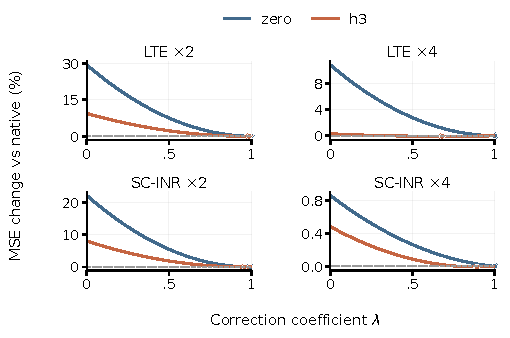
\includegraphics[width=\columnwidth]{figures/attenuation.pdf}
\caption{Complete output-attenuation curves over 32 images and both
seeds. Zero is native mean MSE; lower is better. Dots are exact
HR-informed group optima, not deployable selections. Vertical ranges differ.}
\label{fig:attenuation}
\end{figure}

\textbf{Robustness and visible scale.}
Six fixed conventions cross raw or clipped endpoints with shave0/4/8;
clipping precedes interpolation. All retain mean benefit over zero and
overall harm from half-correction (MSE increases .226--7.67\% across
groups/conventions), although individual labels vary. Most negative RGB
records in Table~\ref{tab:failures} lose at most .01 dB; counts do not
imply large perceptual damage.

\section{Controlled Failure and Allocation Interventions}
\label{sec:controlled}
\subsection{A fixed class of wrong-direction corrections}
At $\times4$, a monochrome HR64 target repeated across RGB is
$t=.5+L+H$. Low modes are $L=\{(2,0),(0,2),(2,2)\}$ and the middle
templates are $\{(10,0),(12,0),(14,0)\}$ and
$\{(10,0),(0,12),(10,10)\}$, in cycles per 64 pixels.
Each cosine amplitude is .04. Periodic separable bicubic-AA $A$ gives
\begin{equation}
 y_\eta=A(.5+L)+\eta A(H),\qquad\eta\in\{0,.5,1\}.
 \label{eq:path}
\end{equation}
Four high-branch phases (zero plus three uniform vectors, seed 20261012)
cross four translations $\{0,.5\}^2$ in LR-pixel units; both branches
translate. High templates use $\{(18,0),(22,0),(26,0)\}$ and
$\{(18,0),(0,22),(18,18)\}$. The low control uses
$\{(4,0),(0,4),(4,4)\}$ and always observes $At$.
The original 240 conditions contain 148 unique inputs, not independent
images. Primary centre32 and sensitivity full64 contain integer periods;
metrics are unclipped, with the same three bands.

For the 32 middle conditions, $\eta:0\to1$ lowers middle-band gain in
29/32 LTE and 32/32 SC cases; alignment changes positive-to-negative in
14/32 and 16/32. The latter 16 define the focal SC class below; all 32
remain in every analysis. Direction/gain tolerances are $10^{-10}/10^{-8}$.
Changing $\eta$ fixes the target but changes LR energy and gradients;
it is not pure aliasing. Equal-target-power phase changes in high
templates produce both gain signs in all eight template--position groups
per model: power alone does not determine benefit. At $\eta=0$, hidden-phase
variants share the same input/output and cannot demonstrate neural
adaptation to hidden phase.

\subsection{Test weight drift, then isolate allocation}
\label{sec:allocation}
The following tests reuse the seen grid and SC seed1 checkpoint; they
are retrospective interventions, not new held-out image tests.
In all 16 focal cases, the old correction remains positively aligned
against the new zero-cell residual, whereas the new correction is
negatively aligned against both residuals. A change in the remaining
error alone therefore does not explain these reversals.
Let $U_i$ be each input's unweighted Fourier/coefficient features at
zero cell, $W_i$ its native sinc weights, and $D$ the fixed MLP.
First cross carriers $U_0/U_1$ and envelopes $W_0/W_1$, keeping recipient
phase, carrier frequency, skip and decoder fixed.
Swapping $W_0$ onto $U_1$ rescues only 1/16 focal negative gains.
This swap does not support envelope drift as a major explanation.
Two controls matched to the $U_1(W_0-1)$ feature-step norm---uniform
attenuation and a fixed paired sine/cosine channel permutation---restore
positive gain in all 16. This donor-norm observation motivates a
separately frozen native-norm confirmation; it does not establish it.

For each $\eta=1$ input, set
\begin{equation}
 \Delta z_n=U\odot(W_1-1),\quad
 \Delta z_u=-\alpha U,\quad
 \alpha=\frac{\|\Delta z_n\|_F}{\|U\|_F}.
 \label{eq:allocation}
\end{equation}
The norm spans four local-ensemble branches, 4096 queries and 256
features: $\|\Delta z_u\|_F=\|\Delta z_n\|_F$. It does not match each
position/channel separately or match RGB correction magnitude.
Both preserve $U$, skip, ensemble weights and MLP parameters.
Their full RGB changes, with branch weights $q_j$, are
\begin{equation}
 d_v=\tfrac12\sum_j q_j[D(U_j+\Delta z_{v,j})-D(U_j)],
 \quad v\in\{n,u\}.
 \label{eq:decode}
\end{equation}
The factor $1/2$ undoes output normalisation; both share the zero-cell
RGB reference. A second response freezes all ReLU masks at $U_j$:
replace the bracket by $J_D(U_j)\Delta z_{v,j}$. This is an exact
fixed-mask affine intervention, not an approximation asserted for the
original nonlinear network. It tests whether gate switching is necessary
for the allocation effect.

\begin{figure*}[t]\centering
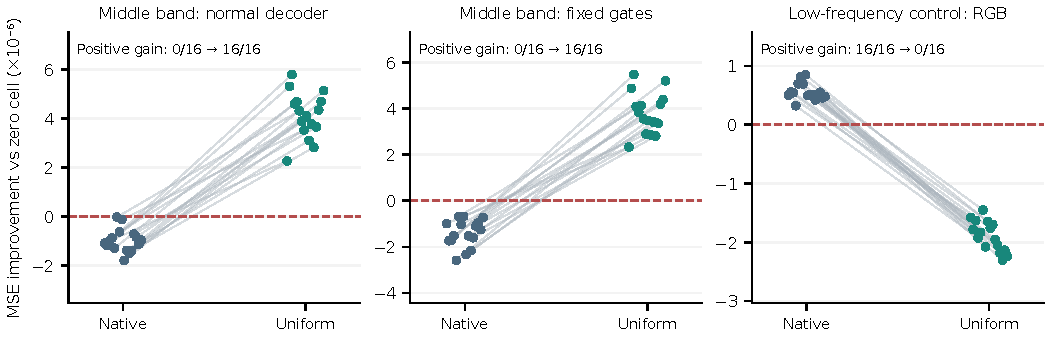
\includegraphics[width=\textwidth]{figures/allocation-confirmation.pdf}
\caption{Same native feature-step norm, different allocation. Each line
is one fixed condition. Left: all 16 focal middle-band corrections switch
from harmful to beneficial. Centre: this persists with zero-cell decoder
gates frozen. Right: all 16 low-frequency controls instead switch from
beneficial to harmful in RGB. All panels use centre32; the first two
score the middle band, the third all RGB. Gain is relative to zero cell;
vertical ranges differ. This is not a general repair.}
\label{fig:allocation}
\end{figure*}

\textbf{Allocation changes the outcome at equal feature-step norm.}
In the focal 16 cases, native and frozen-mask native responses both have
negative direction and gain. Uniform allocation makes both positive in
16/16 (Fig.~\ref{fig:allocation}). Over all 32 middle conditions, both
decoder responses change from 31 negative gains to 32 positive gains.
Relative to native, full64 RGB MSE improves in every focal case, with
median reduction .3996\% ($+.01739$ dB); centre32 RGB medians are
.3724\% and $+.01620$ dB.
Restoration is not confined to the selected band, but its absolute
performance effect remains small.

\textbf{A content-dependent effect, not a replacement algorithm.}
All 16 low controls have positive native centre-RGB gain and negative
uniform gain under both decoder responses. In 11/16 uniform cases the
direction remains positive: overshoot accounts for most control failures.
The intervention isolates allocation across feature/query positions as
an intervenable factor in the specified class, beyond total feature-step
norm and gate switching alone. It does not identify useful individual
channels, establish learned frequencies as true image frequencies, or
show that replacing selective conditioning is generally better.

\section{Scope and Conclusion}
\label{sec:limits}
Natural-image replication supports failure measurements for the declared
LTE lineage and contrasts; the allocation intervention covers one SC
checkpoint, $\times4$ and known synthetic samples. Zero cell is outside
training support. Neither establishes natural-image causal prevalence or
an observation-only selector. HR-assisted decisions are not unbiased risk
estimation under generalized SURE assumptions \cite{eldar2008gsure}.
No matching training was used.
Each allocation stage freezes predictions before scoring; independent
NumPy audits re-score every pixel and verify saved 16-query branch probes,
not every internal feature tensor. The stages take 119.49 and 64.14 seconds
on one CPU thread, without GPU.

Native conditioning can improve averages while individual corrections
overshoot or move away from the target. The controlled SC intervention
goes beyond coexistence: reallocating an equal total feature step restores
a specified failure class, even without ReLU gate changes.
The low-frequency counterexample makes the boundary substantive:
appropriate allocation depends on content and the existing decoder.
The contribution is this bounded diagnosis and intervention evidence,
not a universally effective reconstruction method.

\newpage
\section{Acknowledgments}
Claude and OpenAI Codex assisted with text, analysis code, figures and
record checks. Numerical records were audited; human author review and
responsibility are required before submission.
